\label{chap:results}

This chapter will perfom experiments to find out whether or not
\emph{stacked user modeling} is a viable technique.
We will first explain which evaluation metrics will be used,
and the datasets we will use to test the technique.
Then, we will test each of hypotheses given in Section \ref{sec:hypotheses}.
The next chapter will discuss the implications of these results.


\section{Datasets}

To test our model, we need an applicable dataset with users, items and ratings.
We chose the MovieLens dataset\footnote{
See http://www.grouplens.org/node/73 --- accessed 10.05.2011}.
This dataset is often used to test the performance of recommender systems,
for example in \citet[p9]{Alshamri2008}, \citet[p4]{Lemire2005}, \citet[p1]{Adomavicius2005}
and \citet[p2]{Herlocker2004}.
The dataset consits of a set of users, a set of movies, and a set of movie ratings
on the scale $1$ through $5$, and is available in two sizes:
a set of 100,000 ratings from 943 users on 1,682 movies,
and a set of 1,000,209 ratings from 6,040 users of 3,900 movies.

Each collection comes with meta-data on each user, such as
gender, age and occupation. There is also meta-data on each movie,
such as its title, release date and genre. 
For prediction aggregation, we are only interested in the ratings matrix
extracted from this dataset.
The titles of each movie will be used to experiment with personalized search.

To achieve reliable evaluation results, the dataset should be split into
multiple disjoint subsets, so that we can do cross-validation.
This entails running the same experiments across all the subsets,
and averaging the results.
The MovieLens dataset comes with a preset number of splits for this kind of testing.
In the set with 100,000 ratings, the data is split into five disjoint subsets,
which are again split into training and testing sets:

\begin{equation*}
  D = \{ d_1 = \{base_1, test_1\}, d_2 = \{base_2, test_2\}, ..., d_5 = \{base_5, test_5\} \}
\end{equation*}

Each $base_x$ and $test_x$ are disjoint 80\% / 20\% splits of the data in each subset.
We shall perform five-fold cross-validation across all these sets in our experiments.
This way we can be more certain that our results are reliable,
and not because of local effect in parts of the data.
As previously explained, each $base$ set is further split using bootstrap aggregation,
into random subsets for training each stanard recommender model.
The entire base set is then used to train the aggregation models.
Each corresponding $test$ set is then used to evaluate the performance
of each basic model, and each of the aggregators.


\section{Recommenders}

In addition to the dataset, we need a number of recommender systems
that can predict unknown ratings between users and items.
As we have seen, standard recommenders will be used for both the basic predictions,
and for the accuracy estimations for each basic prediction.

Naturally, we need a number of different recommenders, preferably ones that consider
disjoint patterns in the data. Table \ref{table:results:methods}
gives a short overview of the recommender systems we shall employ.
See Section \ref{sec:recommender} for more information on the different
types of recommenders, and Appendix \ref{appendix:implementation}
for information on how these were implemented in the following experiments.

\subsection{Basic Recommenders}

\begin{table}[t]
  \begin{tabular*}{\textwidth}{ l l l l }
    \toprule
    ~ & \emph{method} &  \emph{algorithm} & \emph{description} \\
    \midrule
    S & svd1          & SVD                   & ALSWR factorizer, 10 features. \\
    S & svd2          & SVD                   & ALSWR factorizer, 20 features. \\
    S & svd3          & SVD                   & EM factorizer, 10 features. \\
    S & svd4          & SVD                   & EM factorizer, 20 features. \\
    S & slope\_one    & Slope One             & Rating delta computations. \\
    S & item\_avg     & Baseline              & Based on item averages. \\ 
    S & baseline      & Baseline              & Basd on user and item averages.\\ 
    S & cosine   	    & Cosine similarity     & Weigted ratings from similar items.\\ 
    S & knn       	  & Pearson Corr.         & Weighted ratings from similar users.\\
    \midrule
    A & median    	  & Aggregation           & Median rating from the above methods. \\
    A & average    	  & Aggregation           & Average rating from the above methods. \\
    A & stacked       & Adaptive agg.         & Accuracy predictions from error models. \\
    \bottomrule
  \end{tabular*}
  \caption[Stacked Modeling Methods]{
    Stacked modeling methods: A short description of each of the recommender methods
    used in our experiment. See Section \ref{sec:recommender} for more information.
    For the SVD methods, the factorizers refers to algoriithms used to factorize the ratings matrix.
    An EM factorizer uses the Expectation-Maximization algorithm to find the factors.
    An ALSWR factorizer performs the same factorization with a least-squares approach \citep{Zhou2008}.
    The number of features refers to the truncation of the factors in order to reduce the taste-space.
  }
  \label{table:results:methods}
\end{table}

As seen in Table \ref{table:results:methods}, we have two types of recommenders:
First, we have the basic recommenders, denoted by \emph{S} in the table.
These recommenders each look at the data in different ways to arrive at predicted ratings.
We chose this wide range of recommenders for just this reason:
as previously explained, the performance of aggregate recommenders
are more dependent on the disimilarity of the basic recommenders
than their individual performance.

Let us briefly explain how each basic recommender works.
The SVD methods look for global patterns in the data 
by reducing the ratings-space into a concept-space.
By reducing this space, the algorithm is able to find
latent relations, such as groups of movies that has the same
rating pattern, or groups of users that often rate in a similar manner.

The Slope One and baseline algorithms look at average
ratings for items and from users, and use these to predict ratings.
The cosine similarity algorithm looks for items that are rated
similarly by the same users, and infers item similarity from this measure.
New ratings are then predicted by taking known ratings of other items,
weighted by their item's similarity to the new item.

The KNN algorithm employs yet another approach. This algorithm,
similar in strategy to the cosine similarity algorithm,
looks for users with similar rating patterns.
The similarity is measured with the Pearson Correlation Coefficient.
Predictions are created by collecting ratings from similar users
of the item in question, weighted by their respective similarity.
See Section \ref{sec:recommender} for more 
detailed information on how these recommenders work. 

\subsection{Stacked Recommenders}

The second type of recommenders are the aggregation methods, 
that combine the result of each of the basic recommender systems.
In addition to our stacked user modeling method
(denoted with the key \emph{stacked} in Table \ref{table:results:methods}),
we have the median- and average-based aggregators.
The median aggregator choses the median value of the predictions
produced by the standard recommenders.
Similarly, the average aggregator takes the mean of the
standard predictions.
While not complex in nature, these methods
will help us see how our method compares to simple, traditional
aggregation techniques.

As explained in Section \ref{sec:usermetamodeling},
any basic recommender system can be used for the stacked user modeling method.
The only difference is how this method is trained:
while the basic methods are trained using the ratings matrix,
the stacked methods are trained using the error model,
as seen in Listing \ref{code:training}.
In other words, we have as many possibilities for choosing
the stacked recommenders as the basic recommenders.

For our experiment, we went with SVD recommenders
for each of the stacked models.
That is, each basic recommender method gets a secondary 
accuracy predicting recommender, which in this case is a 
standard SVD recommender.
The SVD recommender is a natural choice in this case,
since we wish to uncover latent patterns of accuracy
for each model.
Examples of these patterns include groups of items
or users a specific recommender works well for.

The choices of recommenders will be further discussed
in Chapter \ref{chap:discussion}.
For now, let us see how we determined the performance of each method.


\section{Evaluation Strategies}

To evaluate how our model performs, we need a measure
for computing the total error across a large number of predictions.
The canonical measure for estimating the error of a 
predictions from a recommender system
is the \emph{Root mean squared error} (RMSE) measure
(e.g. \citet[p17]{Herlocker2004}, \citet[p13]{Adomavicius2005} and \citet[p6]{Bell2007}).
We shall use this measure to estimate the performance
of our adaptive prediction aggregation algorithms.
The RMSE of a set of estimations $\hat{R}$, 
compared to a set of known ratings $R$, is defined as

\begin{equation*}
  RMSE(\hat{R},R) = \sqrt{E((\hat{R} - R)^2)}
  = \sqrt{\frac{
      \sum_{i=1}^{n} (\hat{R}_i - R_i)^2
    }{
      n
    }},
\end{equation*}

where $n$ is the total number of predictions.
The RMSE combines a set of errors into one single combined error.
A beneficial feature of the RMSE is that the resulting error 
will be on the same scale as the estimations. In other words,
if we are predicting values on the scale $1-5$, the computed error
will be on this scale as well. In this case, an error of $1$
would then say that we are on average $1$ point away from the true 
ratings on our $1-5$ scale.

While the RMSE works well for evaluating scalar predictions,
we need another measure for considering a predicted sorting 
from rank estimation methods.
Here, we are not interested in the predicted scores,
but rather in which position each item appears in a sorted list of results.
This is for instance needed when measuring the performance of a
personalized search engine.
Because of this, we are interested in examining how 
personalization with stacked user modeling affects the rankings
from an IR method.

To answer our three hypotheses, we have performed two experiments.
The first experiment evaluates our method when used for
adaptive prediction aggregation, comparing it to 
the methods given in Table \ref{table:results:methods}.
This will help us answer hypotheses H1 and H2.
The second experiment will evaluate our performance
in adaptive rank aggregation, in order to answer hypothesis H3.
For more information on how the algorithms
in this experiment were implemented, see Appendix \ref{appendix:implementation}.



\section{Adaptive Prediction Aggregation}

\begin{table}[t]
  \begin{tabular*}{\textwidth}{ l p{3cm} p{1.5cm} p{1.5cm} p{1.5cm} p{1.5cm} p{1.5cm} }
    \toprule
      ~ & \emph{method} & 
      $d_1$ & $d_2$ & $d_3$ & $d_4$ & $d_5$ \\ 
    \midrule
    S & svd1          & 1.2389	  & 1.1260	  & 1.1327	  & 1.1045	  & 1.1184	 \\
    S & svd2          & 1.2630	  & 1.1416    & 1.1260	  & 1.1458	  & 1.1260	 \\
    S & svd3          & 1.0061	  & 0.9825	  & 0.9830	  & 0.9815	  & 0.9797	 \\
    S & svd4          & 1.0040	  & 0.9830	  & 0.9849	  & 0.9850	  & 0.9798	 \\
    S & slope\_one    & 1.1919	  & 1.0540	  & 1.0476	  & 1.0454	  & 1.0393   \\
    S & item\_avg     & 1.0713	  & 0.9692	  & 0.9662	  & 0.9683	  & 0.9725	 \\
    S & baseline       & 1.0698	  & 0.9557	  & 0.9527	  & 0.9415	  & 0.9492	 \\
    S & cosine   	    & 1.1101	  & 0.9463	  & 0.9412	  & 0.9413	  & 0.9382	 \\
    S & knn       	  & 1.4850	  & 1.1435	  & 1.1872    & 1.2156	  & 1.2022	 \\
    \midrule                                                                    
    A & median    	  & 0.9869	  & 0.8886	  & 0.8857    & 0.8857	  & 0.8855	 \\
    A & average    	  & 0.9900	  & 0.8536	  & 0.8525	  & 0.8525	  & 0.8519	 \\
    A & stacked       & \textbf{0.9324}	  & \textbf{0.8015}	  & \textbf{0.7993}  & \textbf{0.8238} & \textbf{0.8192} \\
    \bottomrule
  \end{tabular*}
  \caption[Results from Experiment 1]{
    Results from Experiment 1:
    Each cell gives an RMSE value for a method on a subset ($d_x$) of our dataset.
    As these are error measures, on the same scale as our predictions,
    lower values indicate better results. Bold values indicate the best result in each column.
    The first column refers to the type of predictions, either singular (S) or aggregation (A).}
  \label{table:results:e1}
\end{table}

Our first hypothesis, H1, states that:
{
  \itshape
  the accuracy of relevance predictions can be improved
  by blending multiple modeling methods on a per-user and per-item basis.
}
The second hypothesis, H2, states:
{
  \itshape
  an adaptive aggregation method can outperform global and generalized 
  blending methods.
}

In order to verify these hypotheses, we performed adaptive prediction aggregation
through stacked user modeling on the five datasets described in the previous section.
Table \ref{table:results:e1} gives the results from this experiment.
Each cell corresponds to the RMSE values for each dataset,
for each recommender and aggregation approach.
The bottom entry in this table refers to our stacked user modeling method.
As seen in this table, stacked user modeling achieved
lower RMSE values than any of the other applied methods.

Statistics from the results in Table \ref{table:results:e1} 
are given in Table \ref{table:results:e1:sum}.
These values are the minimum, maximum and mean values
for each of the methods. We also include
the standard deviation ($\sigma$) for each method,
across our datasets.
This table confirms the results from the full results table:
Our stacked user modeling approach improves the mean performance
of our system.
The mean performance, along with the standard deviation
are shown in Figure \ref{plot:rmse}.

\begin{table}[t]
  \begin{tabular*}{\textwidth}{ l p{3cm} p{2cm} p{2cm} p{2cm} p{2cm} }
    \toprule
      ~ & \emph{method} & 
      \emph{min} & \emph{max} & \emph{mean} & $\sigma$\\
    \midrule
    S & svd1          & 1.1045	& 1.2389	& 1.1441	& 0.2197 \\
    S & svd2          & 1.1260	& 1.2630	& 1.1605	& 0.2277 \\
    S & svd3          & 0.9797	& 1.0061	& 0.9865	& 0.0991 \\
    S & svd4          & 0.9798	& 1.0040	& 0.9873	& \textbf{0.0924} \\
    S & slope\_one    & 1.0393	& 1.1919	& 1.0756	& 0.2415 \\
    S & item\_avg     & 0.9662	& 1.0713	& 0.9895	& 0.2023 \\
    S & baseline       & 0.9415	& 1.0698	& 0.9738	& 0.2196 \\
    S & cosine   	    & 0.9382	& 1.1101	& 0.9754	& 0.2595 \\
    S & knn       	  & 1.1435	& 1.4850	& 1.2467	& 0.3487 \\
    \midrule            
    A & median    	  & 0.8855	& 0.9865	& 0.9065	& 0.2005 \\
    A & average    	  & 0.8519	& 0.9900	& 0.8801	& 0.2344 \\
    A & stacked       & \textbf{0.7993}	& \textbf{0.9324}	& \textbf{0.8352}	& 0.2225 \\
    \bottomrule
  \end{tabular*}
  \caption[Statistics from Experiment 1]{
      Statistics from Experiment 1: 
      This table shows the minimum, maximum and mean RMSE for each of the methods in Table \ref{table:results:e1}.
      The last column shows the standard deviation ($\sigma$) of each method.
      As before, lower values indicate better results, and bold values
      represent the best result in each column.
    }
  \label{table:results:e1:sum}
\end{table}

\begin{figure}[p]
  \centering
  \subfloat[Experiment 1]{\label{fig:rmse:e1}
\pgfplotsset{width=\textwidth,height=8cm}
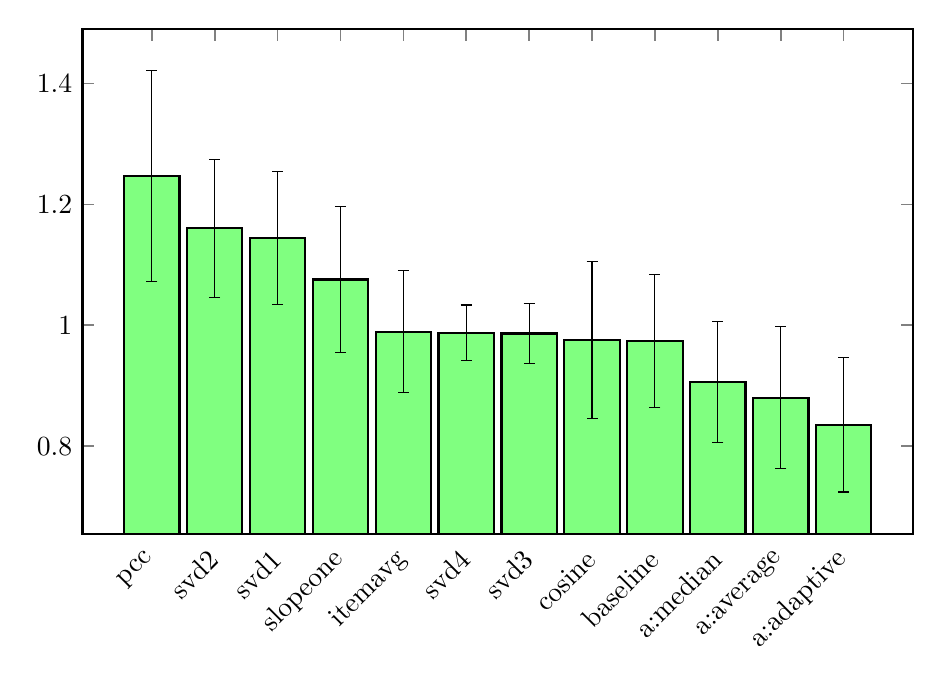
\begin{tikzpicture}
\begin{axis}[
      symbolic x coords={
        pcc,svd2,svd1,slopeone,itemavg,svd4,svd3,cosine,baseline,a:median,a:average,a:adaptive},
      xtick=data,
      x tick label style={rotate=45,anchor=east,yshift=-0.5em,xshift=-0.2em},
      bar width=20pt
    ]
    \addplot [ybar,fill=green!50,error bars/.cd,y dir=both,y explicit] coordinates {
      (pcc, 1.2467) +- (0,0.17435) 
      (svd2, 1.1605) +- (0,0.11385)
      (svd1, 1.1441) +- (0,0.10985)
      (slopeone, 1.0756) +- (0,0.12075)
      (itemavg, 0.9895) +- (0,0.10115)
      (svd4, 0.9873) +- (0,0.0462)
      (svd3, 0.9865) +- (0,0.04955)
      (cosine, 0.9754) +- (0,0.12975)
      (baseline, 0.9738) +- (0,0.1098)
    %};
    %\addplot [ybar,fill=blue!50] coordinates {
      (a:median, 0.9065) +- (0,0.10025)
      (a:average, 0.8801) +- (0,0.1172)
      (a:adaptive, 0.8352) +- (0,0.11125)
    };
\end{axis}
\end{tikzpicture}}

\vspace{1em}
 
  \subfloat[Experiment 2]{\label{fig:rmse:e2}
\pgfplotsset{width=\textwidth,height=8cm}
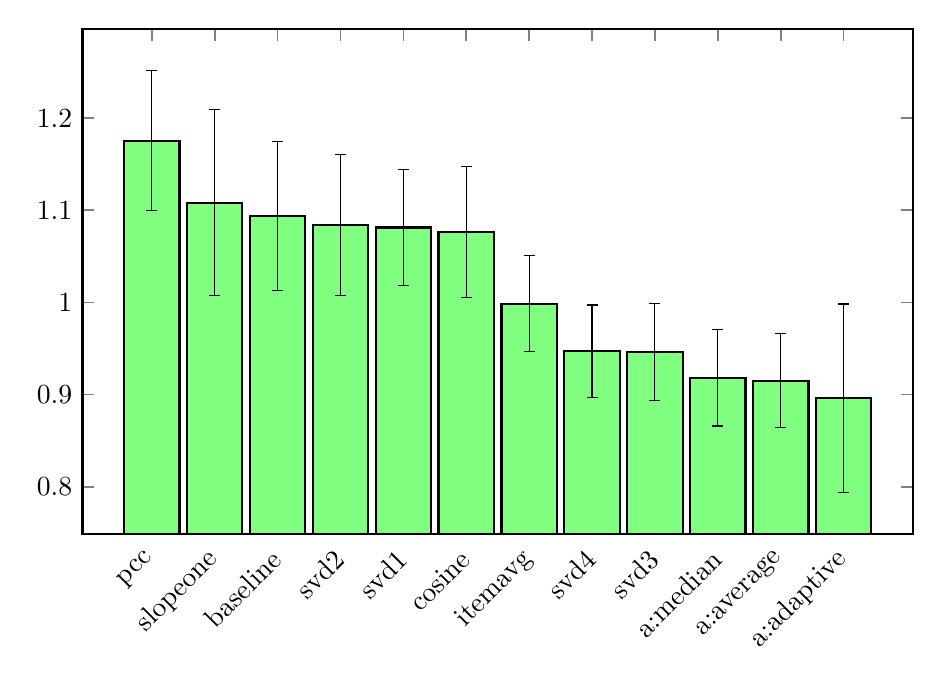
\begin{tikzpicture}
\begin{axis}[
      symbolic x coords={
        pcc,slopeone,baseline,svd2,svd1,cosine,itemavg,svd4,svd3,a:median,a:average,a:adaptive},
      xtick=data,
      x tick label style={rotate=45,anchor=east,yshift=-0.5em,xshift=-0.2em},
      bar width=20pt
    ]
    \addplot [ybar,fill=green!50,error bars/.cd,y dir=both,y explicit] coordinates {
      (pcc, 1.175422) +- (0,0.0758) 
      (slopeone, 1.10813) +- (0,0.101039)
      (baseline, 1.09358) +- (0,0.080985)
      (svd2, 1.084098) +- (0,0.076837)
      (svd1, 1.08128) +- (0,0.063377)
      (cosine, 1.076532) +- (0,0.0709)
      (itemavg, 0.99843) +- (0,0.052021)
      (svd4, 0.947158) +- (0,0.050071)
      (svd3, 0.946024) +- (0,0.052801)
    %};
    %\addplot [ybar,fill=blue!50] coordinates {
      (a:median, 0.918404) +- (0,0.052478)
      (a:average, 0.915036) +- (0,0.051037)
      (a:adaptive, 0.896294) +- (0,0.102056)
    };
\end{axis}
\end{tikzpicture}}

\vspace{1em}

  \caption[Plots of Results for Experiments 1 \emph{\&} 2]{
    Plots of the average RMSEs for Experiments 1 \emph{\&} 2.
    The actual numbers are given in Tables \ref{table:results:e1}
    \emph{\&} \ref{table:results:e2}.
    Note the scale on the y-axis --- the errors are not as pronounced as they might seem. 
  }
  \label{plot:rmse}
\end{figure}




\begin{figure}
\center

\pgfplotsset{width=\textwidth,height=8cm}
\pgfplotsset{every axis/.append style={
thick,
tick style={semithick}}}

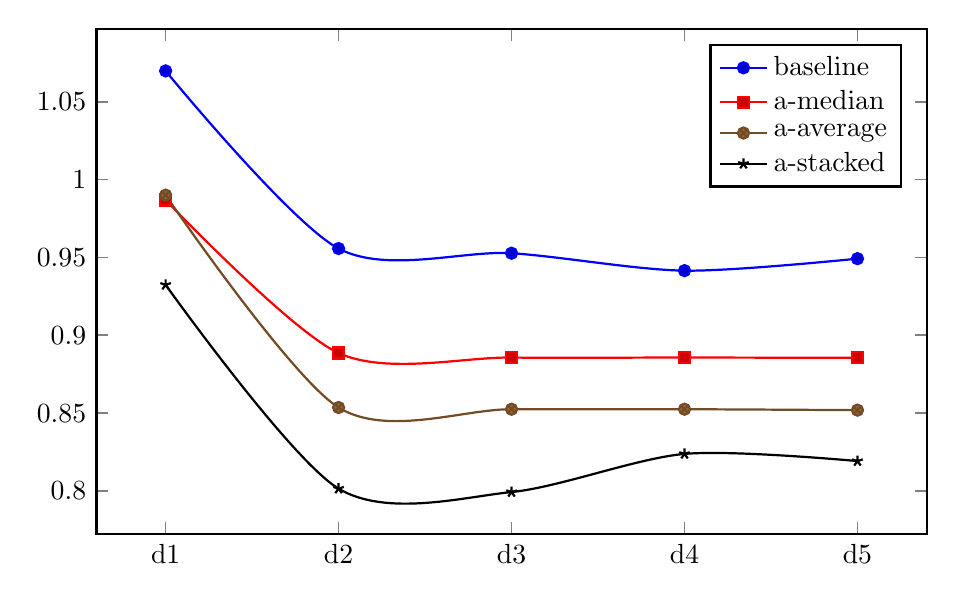
\begin{tikzpicture}

\begin{axis}[
  smooth,
  stack plots=false,
  enlarge x limits=true,
  symbolic x coords={d1,d2,d3,d4,d5},
  xtick=data,
  legend style={
    cells={anchor=west},
    legend pos=north east,
  }
]

\addplot coordinates {
(d1, 1.0698)
(d2, 0.9557)
(d3, 0.9527)
(d4, 0.9415)
(d5, 0.9492)
};
\addlegendentry{baseline}


\addplot coordinates {
(d1, 0.9869)
(d2, 0.8886)
(d3, 0.8857)
(d4, 0.8857)
(d5, 0.8855)
};
\addlegendentry{a-median}
 
\addplot coordinates {
(d1, 0.9900)
(d2, 0.8536)
(d3, 0.8525)
(d4, 0.8525)
(d5, 0.8519)
};
\addlegendentry{a-average}
 
\addplot coordinates {
(d1, 0.9324)
(d2, 0.8015)
(d3, 0.7993)
(d4, 0.8238)
(d5, 0.8192)
};
\addlegendentry{a-stacked}

\end{axis}
\end{tikzpicture}

\caption[RMSE Variations]{
  RMSE Variations: This plot shows that, while the standard deviation of each method may be high,
  this has more to do with the selected dataset than with their performance in comparison with each other.
  The performance of each of the aggregate methods, as well as the best performing standard method,
  follow similar performance paths across the disjoint datasets.
}
\label{plot:datasets}
\end{figure}






Let us take a look at the standard deviation measures from the different methods.
As seen in Figure \ref{plot:rmse}, 
most of the methods, including the stacked models,
exhibit quite a lot of variation in their results.
If these variations occured as a result of unstable
predictions of the same dataset, this would be a substantial problem,
resulting in unreliable predictions.
However, as seen in Figure \ref{plot:datasets},
the standard deviation is mostly caused by the differing
performance across the varying datasets.
As we see, the performance of each of the aggregation methods,
as well as the best performing standard recommender,
follow each other closely. At the same time,
performance varies across the different datasets,
which results in high values for $\sigma$.

What does this mean for hypotheses H1 and H2?
Expressed in terms of this experiment,
H1 posits that stacked user modeling should outperform each of the standard modeling methods
in Table \ref{table:results:e1}.
The adaptive methods blend the results of multiple predictors by estimating the accuracy
on a per-item and per-user basis, satisfying the formulation of H1.

By outperform we mean that our model should have a lower
mean RMSE score than the other singular methods. As we can see in Table \ref{table:results:e1:sum},
\emph{H1 is confirmed for these methods and this dataset}.
While we can not generalize too much on this basis, 
the fact that this dataset is a common testing ground for recommender systems,
that RMSE is the de facto measure for determining performance,
and because of our 5-fold cross-validation, the results allow us 
to confirm hypothesis H1 in these conditions, and likely for other, similar scenarios.
We shall discuss this in Chapter \ref{chap:discussion}.

Similarly, expressed in the same terms, H2 posits that 
our stacked user modeling should outperform the aggregation approaches
given in Table \ref{table:results:e1}.
The \emph{median} and \emph{average} aggregation methods
serve as globalized and generalized aggragation methods,
Stacked user modeling is adaptive in that each prediction is 
aggregated based on the current user and item,
satisfying the language of H2.

As we can see in Table \ref{table:results:e1:sum},
\emph{H2 is confirmed for these methods and this dataset}.
However, as our collection of aggregation methods is a lot simpler
than our collection of recommender systems, the strength of this combination
is notably weaker than that of H1.
Still, the fact that stacked user modeling outperforms these simple aggregation
approaches is a positive result warranting further experiments.
This will also be discussed in Chapter \ref{chap:discussion}.

It would seem then that, based on our experiments, available data
and assumptions of evaluation measures, both H1 and H2 are confirmed.
Our adaptive aggregation approach outperforms both standard recommender
methods and simple generalized aggregation methods.
Notably, our approach is more complex than the methods it outperforms,
so the question whether the methods performance is worth its extra complexity becomes important.
We shall discuss this, and other implications of these results in the next chapter.
For now, let us proceed to the second experiment and hypothesis H3.


\section{Adaptive Rank Aggregation}

Test H3

\begin{table}[t]
  \centering 
  \begin{minipage}{0.49\textwidth}
    \centering 
    \begin{tabular*}{\textwidth}{ l l }
      \toprule
      \emph{\#} & \emph{title}\\
       \midrule
        1 & The Endless Summer 2 \\
        2 & Indian Summer \\
        3 & An Unforgettable Summer \\
        4 & Last Summer in the Hamptons \\
        5 & It's a Wonderful Life \\
        6 & Boys Life \\
        7 & A Life Less Ordinary \\
        8 & Life with Mikey \\
        9 & Country Life \\
        10 & The Low Life \\
        \bottomrule
      \end{tabular*}
    \end{minipage} 
    \hfill 
    \begin{minipage}{0.49\textwidth}
      \centering 
      \begin{tabular*}{\textwidth}{ l l l }
        \toprule
        \emph{\#} & \emph{title} & $\Delta$ \\
        \midrule
        1 & It's a Wonderful Life       & \color{green} $\uparrow$ 4  \\
        2 & The Endless Summer 2        & \color{red} $\downarrow$ 1  \\
        3 & The Low Life                & \color{green} $\uparrow$ 7  \\
        4 & A Life Less Ordinary        & \color{green} $\uparrow$ 3  \\    
        5 & Indian Summer               & \color{red} $\downarrow$ 3 \\
        6 & Country Life                & \color{green} $\uparrow$ 3  \\    
        7 & An Unforgettable Summer     & \color{red} $\downarrow$ 4  \\
        8 & Boys Life                   & \color{red} $\downarrow$ 2  \\    
        9 & Last Summer in the Hamptons & \color{red} $\downarrow$ 5  \\
        10 & Life with Mikey            & \color{red} $\downarrow$ 2   \\
      \bottomrule
    \end{tabular*}
  \end{minipage} 
  \vspace{1em}
  \caption[Adaptive Rank Results]{
    Adaptive rank results:
    These tables show two sets of results for the query "summer life", in our MovieLens dataset.
    The left table shows the ranking as returned by the IR model.
    The right table shows the re-ranked results when their scores
    are combined with the stacked user modeling scores,
    as per Listing \ref{code:rank:prediction}.
  }
  \label{table:foobar}
\end{table}


%\section{Results}
%Summarize results


